\question
(0,5 балла) Друг кота Степана, кот Антоний, тоже захотел заняться творчеством. Но до рисования ему пока далеко, он научился рисовать только палочки и точки. Помогите коту Антонию нарисовать свой автопортрет. Вам нужно нарисовать эквивалентный граф для рисунка Антония в планарной укладке и в виде кота (чтобы было похоже на Антония). А также Антоний изучает дискретную математику, помогите ему разобраться.

Рисунок Антония:
\begin{minipage}[h]{0.45\linewidth}
\center{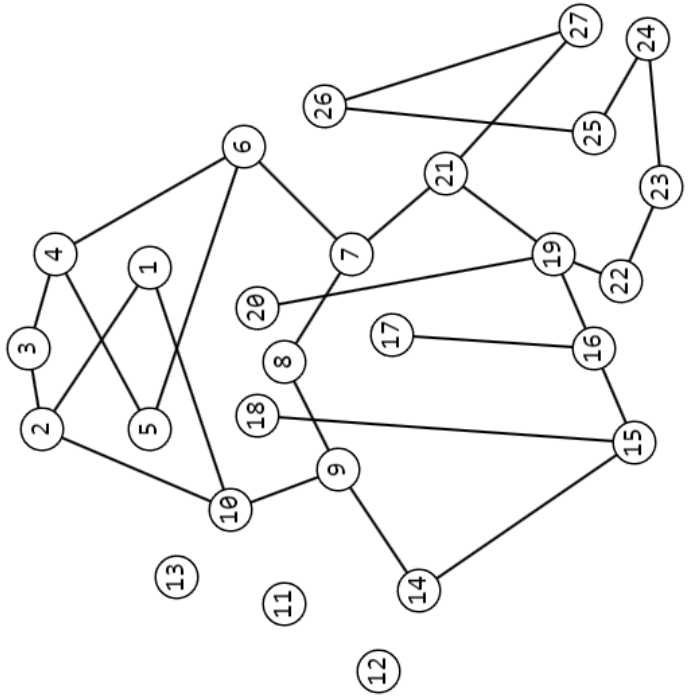
\includegraphics[width=0.7\textwidth]{pic/21.png} }
\end{minipage}

Задания для этого графа:
\begin{enumerate}
\item Выделите блоки и точки сочленения.
\item Выделите компоненты реберной двусвязности и мосты.
\item Сколько висячих вершин?
\item Сколько изолированных вершин?
\item Сколько простых циклов?
\end{enumerate}

---------------

Автор -- Алёна Холмогорова, M3302
